\documentclass[12pt,fleqn]{article}
\usepackage[utf8]{inputenc}
\usepackage[T1]{fontenc}
\usepackage{palatino}
\usepackage{graphicx}
\usepackage{verbatim}
\usepackage[german]{babel}
%\usepackage[a4paper]{geometry}
\usepackage[a4paper, top=2cm, bottom=2cm, left=1.5cm, right=1.5cm]{geometry}
\usepackage{amsmath, amsthm, amssymb, amsfonts}
\usepackage{listings} 
\usepackage{pgfplots}
\usepackage{xcolor}
%\usepackage[dvipsnames]{xcolor}

\usepackage[gen]{eurosym}
\DeclareUnicodeCharacter{20AC}{\euro{}}

%\usepackage[pdfborder={0 0 0}]{hyperref}

%\usepackage{tikz}
%\usetikzlibrary{intersections}

\usepackage{tabularx}
\usepackage{longtable}

\usepackage{parskip}
\setlength{\parindent}{0pt}
\setlength{\mathindent}{0pt}

\usepackage{enumitem}
%\setlist{nolistsep,topsep=0pt,partopsep=0pt}
%\setlist{notopsep}

% für MA: %
\usepackage{multirow}
\usepackage{fancyvrb}
\usepackage{tikz,lipsum,lmodern}
\usepackage[most]{tcolorbox}
\usepackage{float}
\usepackage[german]{struktex}

\pgfplotsset{compat=1.18}

% nur für Draft-Zitierungen %
\usepackage{natbib}

%\newcommand{\rom}[1]{\uppercase\expandafter{\romannumeral #1\relax}}

\begin{comment}
\usepackage{listings}
\lstset{
basicstyle=\small\ttfamily,
columns=flexible,
breaklines=true
}
\end{comment}

\begin{comment}
\usepackage{fancyvrb}
% redefine \VerbatimInput
\RecustomVerbatimCommand{\VerbatimInput}{VerbatimInput}%
{fontsize=\scriptsize,
 %
 frame=lines,  % top and bottom rule only
 framesep=2em, % separation between frame and text
% rulecolor=\color{Gray},
 %
 label=\fbox{data.txt},
 labelposition=topline,
 %
 commandchars=\|\(\), % escape character and argument delimiters for
                      % commands within the verbatim
 commentchar=*        % comment character
}
\end{comment}

\pagestyle{empty}



\begin{document}

\section{Symfony}

\subsection{Controller}

Routing

\subsection{Serializer}

XML

CSV

SQL-Insert

\subsection{Console}

\subsection{Template-Engine Twig}

\subsection{Http Foundation}

Request

Response

StreamedResponse

\subsection{HttpClientInterface}

Download

\subsection{File System}

\subsection{UUID}

\section{Backend}

\subsection{Setup-XML}

\subsection{Konsole}

\subsection{Doctrine}

\subsection{Datenbank / MySQL}

\section{Frontend}

\subsection{Webpack / Node.js}

\subsection{Bootstrap}

Layout, Nav-Tabs, Modal, Icons

\subsection{SCSS}

\subsection{Tooltips}

\section{AJAX}

Modal

BfArM/Dimdi Links

\section{}

\newpage 
% Version Control: thomas2019pragmatic (data1)

Model-View-Controller \citep[Seite 176f]{voorhees2020guide}

\begin{figure}[H]
    \centering
    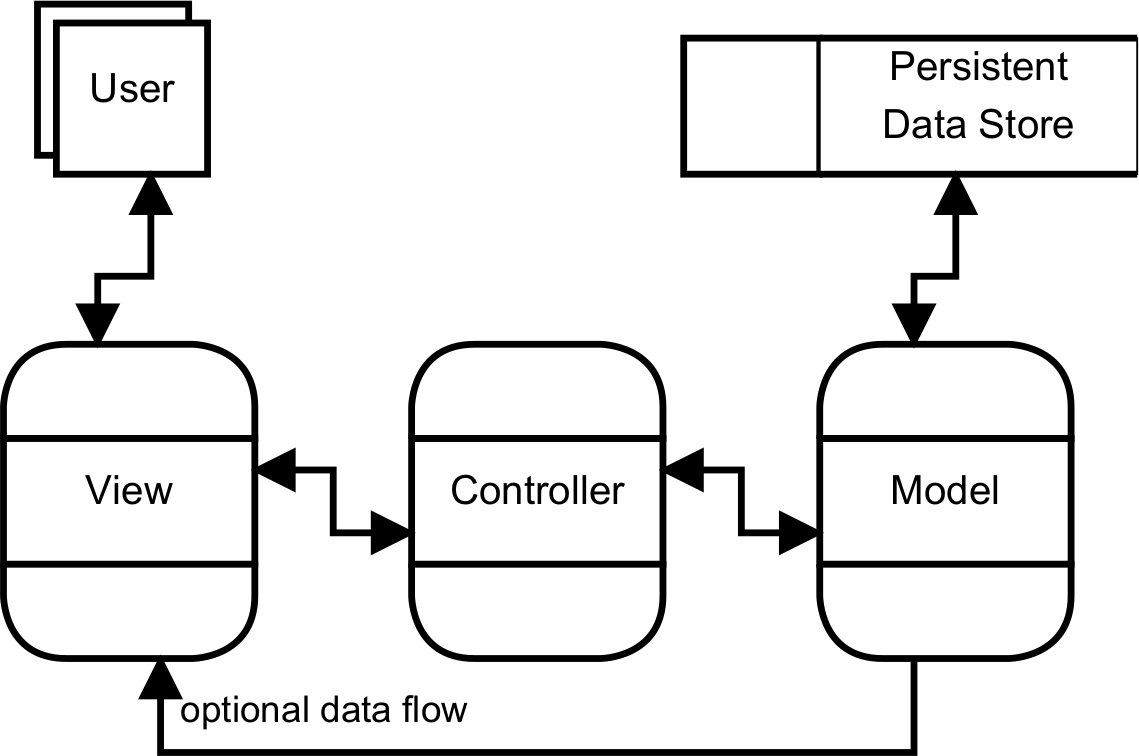
\includegraphics[width=.7\linewidth]{../img/mvc.png}
    \caption{\citep[Seite 177]{voorhees2020guide}}
\end{figure}

Abstraction and Decoupling

Symfony \citep{potencier2022symfony}

Dependency Injection \citep{seemann2019dependency}

When to stream? \citep{braaksma2014streaming}

CSS Flexbox \citep{flexbox-csstricks}

Programming Languages Harmful \citep{janssenscan}

\section{Anonyme Funktionen}

Callback

Zum Schreiben der ConceptMap

Data-Preprocessing

InsertEncoder



https://dev.mysql.com/doc/refman/en/insert-optimization.html

\bibliographystyle{IEEEtranSN}
\bibliography{tech}

\end{document}
